\chapter{Process}

\section{Process capturing}
The as-is / current process has been reverse engineered based on the documents, regulations and policies that the finance administration UZH provides to the finance administrations at the individual departments. Moreover also several semi-structured and informal interviews with Claudia Leibundgut from the finance administration IFI and with researchers at the Communication Systems Group (CSG) have been conducted.\par
The emerged process has then been digitally enabled and validated again in collaboration with Claudia Leibundgut (representative for the finance administration IFI) and Thomas Bocek (representative for the CSG).

\section{Digitally enabled reimbursement process}
\label{sec:processflow}
The process starts in the lane \textit{Expense Creator}; an expense is created, receipts are added and the expense as a whole is forwarded to the next higher instance for verification. After the verifications by the \textit{Manager} or its \textit{Deputy} and by the \textit{Finance administration IFI} are successful, the signing-process will start.\newline
During the signing-process, all three entities, namely the \textit{Expense Creator}, the \textit{Manager / Deputy} and the \textit{Finance administration IFI} need to sign the document. All entities can only sign with the same type of signing, i.e. all digitally or all electronically. If all of them have signed the document, the \textit{Expense Creator} can print the expense and hand it over physically to the \textit{Finance administration IFI}.\newline
Since this part of the process is still performed manually, Claudia Leibundgut proposed that the Expense Creators should send the post-mail directly to the Finance administration of UZH. This bears the risk that manipulations by the Expense Creators go unnoticed.\newline
At the point of printing, the sub-process "expense-creation" is at its end and all further activities are out of scope of the reimbursement tool, as it is specified in the project scope. The chapter \ref{sec:future-work} offers further improvements to the current, and even more important, to the part of the process that currently is out of scope. To name an example, all of the expense receipts will be printed and after verification through the \textit{Finance administration UZH} they will be digitalized again. This media disruption could be resolved by extending our tool.\par

This new process implies certain roles and states. These are further described in section \ref{sec:states} and \ref{sec:user-roles}
\newline


\subsection{Corner Cases}
If a \textit{Manager} will act as a \textit{Expense Creator} the expense will only be submitted to the \textit{Finance administration} for approval. During the signing-process, the \textit{Manager}'s manager has to sign as a higher authority.\newline
Analogous if the \textit{Expense Creator} is \textit{Finance administrator IFI}, \textit{Department Manager} or \textit{Head of Institute}.\par 
At this point, an illustrative step-through my be clarifying:
	
	\begin{itemize}
		\item \textbf{Step-Through:} (create) - (validate) - (sign) - (sign) - (sign)
		\item \textbf{Prof:} Prof - Fadmin IFI - Prof - Depman - Fadmin IFI
		\item \textbf{Depman:} Depman - Fadmin IFI - Depman - Headinst  - Fadmin IFI
		\item \textbf{Headinst:} Headinst - Fadmin IFI - Headinst - Depman - Fadmin IFI	
	\end{itemize}
	
Another corner case are finance administration personnel: Here, after the creation of the expense, the expense is sent straight to the finance administration's "expense pool". In the case of finance administrators submitting their expenses to the pool, of course these expenses cannot be self-assigned and only validated by other finance administrator but not themselves.

\begin{itemize}
	\item \textbf{Fadmin:} fadmin1 ifi - fadmin2 ifi - fadmin1 ifi - depman - fadmin2 ifi
\end{itemize}


\newpage
\subsection{Process diagram}
\label{sec:process-diagram-rotated}
	\begin{figure}[H]
		{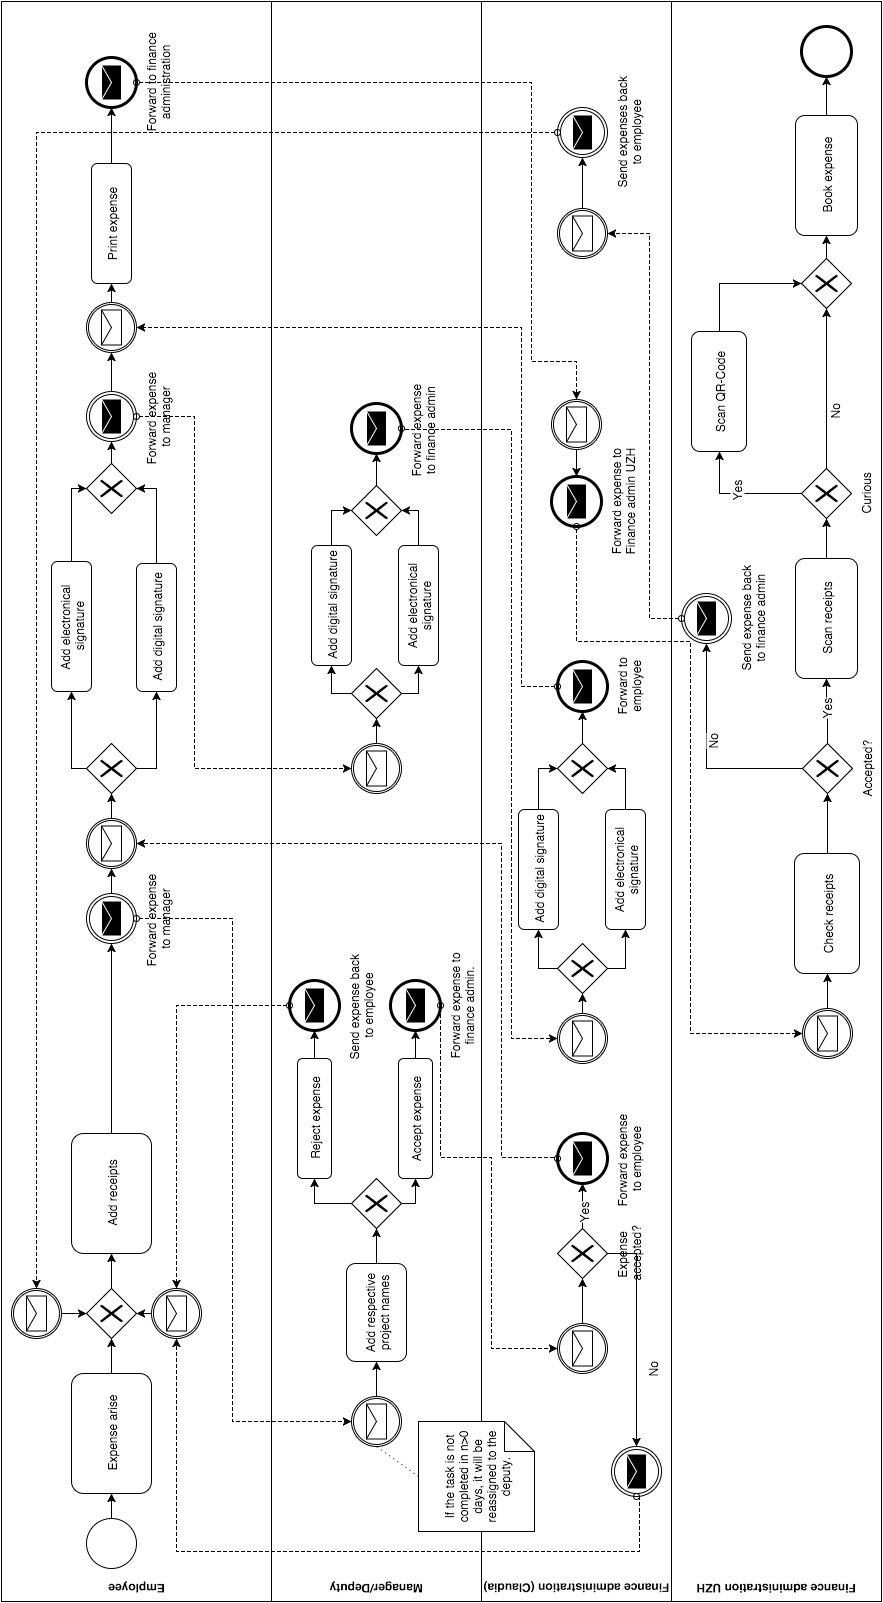
\includegraphics[width=0.75\textwidth]{process-diagram-rotated}}
	\end{figure}
\newpage

\subsection{States}
\label{sec:states}
During the process an expense passes through various states. An expense is always in one and only one of the states defined in the following section. The State-diagram in \ref{sec:state-diagram} visualizes the pass through graphically. Users have different roles and therefore also different competencies to modify the state of an expense.

\begin{itemize}
	\item \textbf{DRAFT} state occurs if the expense is created and yet has not been assigned to a \textit{Manager}.
	
	\item \textbf{TO\_BE\_ASSIGNED} state occurs if the expense is submitted, but has not been assigned to a specific manager or the \textit{Finance administration} user. If the expense has been assigned, the expense will either have the state \newline \textbf{ASSIGNED\_TO\_MANAGER} or \newline \textbf{ASSIGNED\_TO\_FINANCE\_ADMIN}.
	
	\item \textbf{ASSIGNED\_TO\_MANAGER} state occurs if the expense is assigned to a specific \textit{Manager}.
	
	\item \textbf{ASSIGNED\_TO\_FINANCE\_ADMIN} state occurs if the expense is assigned to a specific \textit{Finance admin}.
	
	\item \textbf{REJECTED} state occurs if the created expense is not accepted by the \textit{Manager}, \textit{Department manager} or the \textit{Finance administration}. In \textbf{REJECTED} state the expense will be reassigned to the user who created it.
	
	\item \textbf{SIGNED} state occurs if the expense has been signed by all participants; \textit{Expense Creator}, \textit{Manager} or \textit{Department manager} and \textit{Finance administration}. There exist sub states that occur if the expense is in the process of being signed:
	\begin{itemize}
		\item \textbf{TO\_BE\_SIGNED\_BY\_USER} occurs if the expense needs to be signed by the \textit{Expense Creator}.
		\item \textbf{TO\_BE\_SIGNED\_BY\_MANAGER} occurs if the expense needs to be \newline signed by the \textit{Manager}.
		\item \textbf{TO\_BE\_SIGNED\_BY\_FINANCE\_ADMIN} occurs if the expense \newline needs to be signed by an user with role \textit{Finance administration}.
	\end{itemize}
	
	\item \textbf{PRINTED} state occurs if the expense and all its receipts are successfully converted into a digital document.
	
	\item \textbf{ARCHIVED} state occurs if the expense has been printed.
\end{itemize}

The names of the various states are coupled with the user roles. For example \textbf{ASSIGNED\_TO\_FINANCE\_ADMIN} implies that the expense is assigned to a user with role \textit{Finance Administration}.
\newpage

\subsection{State diagram}
\label{sec:state-diagram}

\begin{figure}[H]
	{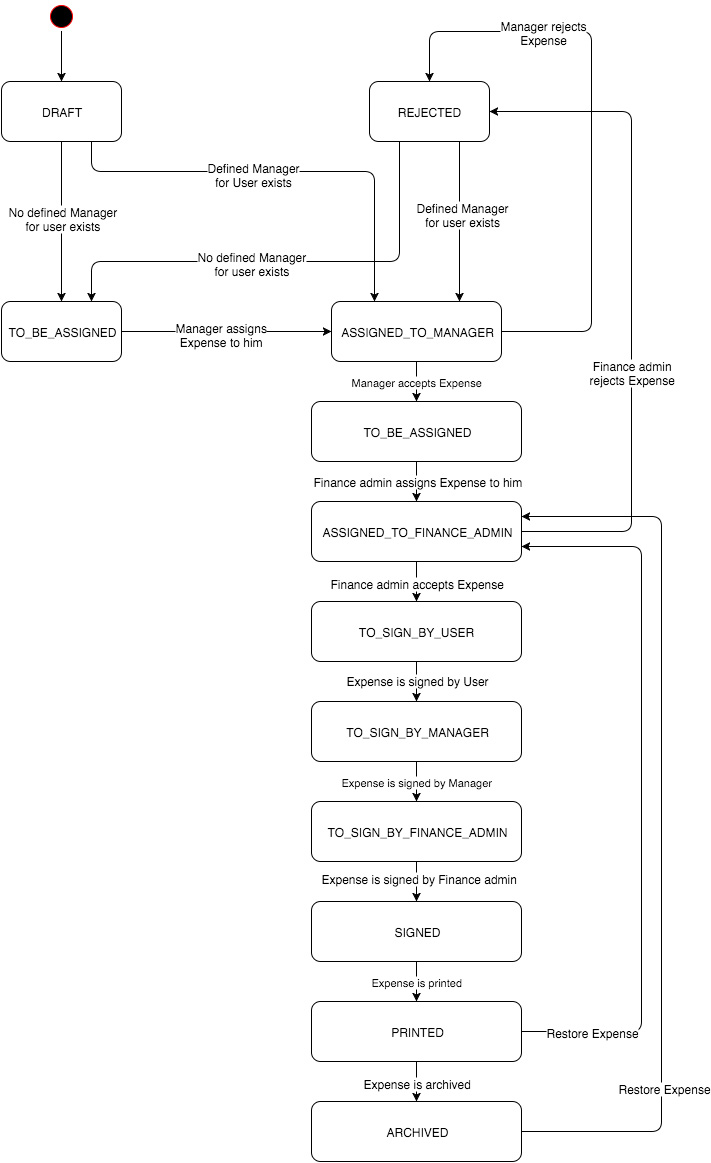
\includegraphics[width=0.8\textwidth]{state-diagram}}
\end{figure}
\newpage

\section{User roles}
\label{sec:user-roles}

The system maps the users available in the IFI LDAP server. So every user that exists in the LDAP is capable to login to the system. He can use the same user name and password that he uses for the other University of Zurich services for login. \par

The reimbursement-tool provides different user roles. Also the roles on the reimbursement-tool are mapped with the LDAP user roles of the University of Zurich. So a user who is defined as professor for a specific group on the LDAP will be the manager for all users of this group. The reimbursement-tool provides the roles with the following authorizations to alter expenses:

\begin{itemize}
	\item \textbf{Unregistered user} are users, who are authorized to login the reimbursement-tool but have not yet completed the registration process. They have only access to the public REST services (see \ref{sec:rest-services}).
	\item \textbf{Registered user / User} passed the registration process. He can access the reimbursement-tool and create and manage his created expenses. He has one of the following roles:
	
	\begin{itemize}
		\item \textbf{Expense Creator} is authorized to create and edit expenses as long as they are in DRAFT state.
		
		\item \textbf{Manager / Professor} are authorized to reject, accept and edit expenses as long as it is assigned to him.
		
		\item \textbf{Department manager} has the same authorizations as the \textit{Manager}. If a \textit{Manager} is outreach, his assignments will be forwarded to the respective \textit{Department manager}.
		
		\item \textbf{Finance administration} is authorized to reject, accept and edit expenses once they have been accepted by a \textit{Manager} or \textit{Department manager}. Furthermore they can manage the available cost categories and search for expenses.
		
		\item \textbf{Head of institute} has the same authorizations as the \textit{Manager}. In contrast to the \textbf{Department manager} there exists only one user that can be \textit{Head of institute}. The \textit{Head of institute} will have to approve the expense if, for any reason the \textit{Department manager} is not available.
	\end{itemize}
\end{itemize}
